\chapter{Evaluation}\label{chap:Evaluation}
This section evaluates how successfully and effectively the implemented features achieve the goals stated in the introduction.

\section{Success}
This evaluation is more ambitious than that presented in the project proposal goals. As demonstrated below, the type witness search procedure and cast slicing features exceeds all core goals\footnote{That is, reasonable coverage and performance.} presented in the project proposal, while type slicing had not been conceived, but naturally complements cast slicing. Some extension goals were reached: almost of Hazel was supported\footnote{Except the type slicing of two constructs: type functions and labelled tuples (which was a new feature merged by the Hazel dev team in February).}. The search procedure was not mathematically formalised, but the slicing mechanisms were.

\section{Goals}\label{sec:EvaluationGoals}
This project devised and implemented three features: \textit{type slicing, cast slicing,} and a \textit{static type error witness search procedure}. Each of which had a clear intention for it's use:

\paragraph{Type Slicing:} Expected to give a greater static context to expressions. Explaining why an expression was given a specific type.

\paragraph{Cast Slicing:} Expected to provide static context to runtime type casts and propagate this throughout evaluation. Explaining where a cast originated and why it was inserted.

\paragraph{Search Procedure:} Finds dynamic type errors (cast errors) automatically, linked back to source code by their execution trace and \textit{cast slice}. Therefore, a static type error can be associated automatically with a concrete dynamic type error \textit{witness} to better explain.

\section{Methodology}\label{sec:EvaluationMethodology}
I evaluate the features and their various implementations (where applicable) along \textit{four} axes. With quantitative measures were evaluated over a corpus of ill-typed and dynamically-typed Hazel programs (\cref{sec:EvaluationCorpus}):

\subsubsection{Quantitative Analysis}
\paragraph{Performance: } \textit{Are the features performant enough for use in interactive debugging? Which implementations perform best?}

The time and space usage of the search procedure implementations were micro-benchmarked for each ill-typed program in the corpus. Up to 100 runs were taken per program with estimated time, major and minor heap allocations were estimated using an ordinary linear regression (OLS) to $r^2 > 0.95$\footnote{TODO: get values} via the \textit{bechamel} library \cite{Bechamel}.

\paragraph{Effectiveness: } \textit{Do the features effectively solve the problems? Are the results easily interpretable by a user?}

The \textit{coverage},  what proportion of programs admit a witness, for each search procedure implementation was measured. The search procedure does not always terminate, a 30s time limit was chosen. The coverage was expected to be \textit{reasonable}, chosen at 75\%.

Additionally, the \textit{size} of witnesses, evaluation traces, type slices, and cast slices were measured. The intention being that a smaller size implies that there is less information for a user to parse, and hence easier to interpret.\footnote{Not necessarily \textit{always} true, but a reasonable assumption.}

\subsubsection{Qualitative Analysis}
\paragraph{Critical: } \textit{What \textit{classes} of programs are missed by the search procedure? What are the implications of the \textit{quantitative} results? What improvements were, or could be made in response to this?}

This section provides \textit{critical} arguments on {usefulness} or {effectiveness}, which are \textit{evidenced} by quantitative data. Differing implementations and \textit{subsequent improvements}\footnote{Which were then implemented and analysed.} are compared. Additionally, further unimplemented improvements are proposed.

\paragraph{Holistic: } \textit{Do the features work well together to provide a helpful debugging experience? Is the user interface intuitive?}

Various program examples are given, demonstrating how all three features can be used together to debug a type error. Improvements to the UI are discussed.\footnote{Improved UI being a low-priority extension.} 



\section{Hypotheses}
Various hypotheses for properties of the results are expected. The evidence and implications of these are discussed in the \textit{critical evaluation}.

\paragraph{Search method space requirements: } The space requirements for DFS and Bounded DFS are expected to be lower than that of BFS and interleaved DFS.

\paragraph{Contribution slices are large: } Contribution slices highlight all static regions of a program. This likely shows \textit{too much} information to the user at once. The other slicing methods (synthesis, analysis, ad-hoc) are expected to produce significantly \textit{smaller} slices. 

\paragraph{The Small Scope Hypothesis: }
\label{sec:SmallScopeHypothesis} This hypothesis \cite{SmallScopeHypothesisOrigination} states that a high proportion of errors can be found by generating only \textit{small} inputs. Evidence that this hypothesis holds has been provided for Java data-structures \cite{SmallScopeHypothesis} and answer-set programs \cite{SmallScopeHypothesisAnswerSet}. Does it also hold for finding dynamic type errors from small \textit{hole instantiations}?

\paragraph{Smaller instantiations correlate with smaller traces: } As functional programs are often written recursively, destructuring compound data types on each step. If this and the small scope hypothesis hold, then most errors could be found with \textit{small execution traces}.

\section{Program Corpus Collection}\label{sec:CorpusCollection}

A corpus of small and mostly ill-typed programs was produced, containing both dynamic (unannotated) programs and annotated programs (containing statically caught errors). We have made this corpus available on GitHub \cite{HazelCorpus}.

\subsection{Methodology}
There are no extensive existing corpora of Hazel programs, nor ill-typed Hazel programs. Therefore, we opted to transpile parts of an existing OCaml corpus collected by Seidel and Jhala \cite{OCamlCorpus}. Which is freely available under a Creative Commons CC0 licence. 

I am grateful for my supervisor who created a best-effort OCaml to Hazel transpiler \cite{HazelOfOCaml}. This translates the OCaml examples into both a dynamic example, and a (possibly partially) statically typed version according to what type the OCaml type checker expects expression to be.\footnote{The annotations may be consistent, as we are translating ill-typed code.}

This corpus contains both OCaml unification and constructor errors. When translated to Hazel, these may manifest as differing errors. The only errors that the search procedure is expected to detect are those which contain \textit{inconsistent expectations} errors. Hence, the search procedure is ran on the corpus of annotated programs filtering those without this class of errors. Additionally, the search procedure requires the erroneous functions to have holes applied to start the search, these are inserted automatically by the evaluation code after type checking the programs.


\subsection{Statistics}
The program corpus contains \textbf{698} programs of which \textbf{203} were applicable to performing the search procedure on. Averages and standard deviations in size and trace size\footnote{When using normal, deterministic, evaluation.} shown in \cref{fig:CorpusStats}.
\begin{figure}
\centering
\begin{tabular}{c|ccccc}
& \textbf{Count} & \multicolumn{2}{c}{\textbf{Prog. Size}}& \multicolumn{2}{c}{\textbf{Trace Length}}
&  && Avg. & Std. dev. & Avg. & Std. dev.\\
\hline
\textbf{Unannotated} &404 &117 &81 &9&9\\
\textbf{Annotated} &294 &117 &76 &9&9\\
\textbf{Searched} &203 &120 &77 &10 &10\\
\hline
(Total)  &698 &117 &79 &9 &9\\
\end{tabular}
\caption{Hazel Program Corpus}
\label{fig:CorpusStats}
\end{figure}

\section{Performance Analysis}\label{sec:PerformanceAnalysis}

\subsection{Slicing}
The type and cast slicing mechanisms don't increase the time complexity of the type checker nor evaluator. Hence, they are still as performant as the original, and can still be used interactively in the web browser up to medium sized programs.

\subsection{Search Procedure}
Only the annotated ill-typed corpus containing inconsistency errors are used in evaluating the search procedure. After all, any well-typed program cannot have a dynamic type error.

As the search procedure may be non-terminating, the results are found under a 30s time limit. Each search implementation gives terminates on a different set of programs with potentially different witnesses and traces. The succeeding \textit{effectiveness} analysis considers the search procedures results under these constraints.

However, by micro-benchmarking only the programs which do not time-out, the time and space used searching for each witness can be estimated. The averages over all successful programs for each implementation are given in \cref{fig:SearchPerformance}. These results suggest that, as expected, BFS and interleaved DFS (IDFS) use more memory in total\footnote{Although, IDFS efficiently keeps most memory allocated short lived, being in the \textit{minor} heap.} than bounded DFS (BDFS) and DFS, while DFS is the fastest\footnote{Having the least overhead.}. 

This is not a fair test as the sets of programs averaged over are different, for example, BFS only succeeds on the smaller programs. Hence, the ratios between each implementation as compared to DFS on only the programs which \textit{both} succeed on are given in \cref{fig:SearchPerformanceRatios}. Under this, the results are even more pronounced.
\begin{figure}
  \centering
  \begin{tabular}{lc|cccc}
  & Averages & \multicolumn{4}{c}{\textbf{Implementations}}\\
   & unit & \texttt{DFS} & \texttt{BDFS} & \texttt{IDFS} & \texttt{BFS}\\
   \hline
   \textbf{Time} & ms &  7.6 & 73 & 140 & 120\\
   \textbf{Major Heap} & mB & 3.7 & 32 & 5.9 & 25\\
   \textbf{Minor Heap} & mB & 66 & 680 & 1900 & 1300
  \end{tabular}
  
\caption{Benchmarks: Search Implementations}
\label{fig:SearchPerformance}
\end{figure}
\begin{figure}
  \centering
  \begin{tabular}{l|ccc}
  Ratios & \multicolumn{3}{c}{\textbf{Implementations}}\\
    vs. \texttt{DFS}& \texttt{BDFS} & \texttt{IDFS} & \texttt{BFS} \\
   \hline
   \textbf{Time} &  8.3 & 52 & 230\\
   \textbf{Major Heap} & 9.0 & 3.2 & 270\\
   \textbf{Minor Heap} & 9.7 & 83 & 390
  \end{tabular}
  
\caption{Benchmarks: Performance ratios to DFS over common programs}
\label{fig:SearchPerformanceRatios}
\end{figure}


\section{Effectiveness Analysis}\label{sec:EffectivenessAnalysis}


\subsection{Slicing}
\textit{Type slice} sizes were calculated by the type checker over the entire corpus, where the size is the number of constructs highlighted. While \textit{cast slice} sizes were calculated over in the elaborated expressions after type checking.

\Cref{fig:TypeSlicingEffectiveness} shows that both type and cast slices are generally small. In particular, the proportion of the context\footnote{Calculated by close approximation by the \textit{program size}. As each program in the corpus is just one definition. Calculating the context itself is non-trivial.} highlighted is very low, generally less than 5\% for dynamic code and 10\% for annotated code. Therefore, they concisely explain the types. However, some slices are still large, as seen by the relatively large standard deviations.

Additionally, for errors, there will be multiple inconsistent slices involved. \Cref{sec:SlicingAnalysis} describes how these slices can be summarised to only report the inconsistent parts. We find that these \textit{minimised} error slices are significantly (3x) smaller than directly \textit{combining} the slices.

\begin{figure}[h]
  \centering
  \begin{tabular}{lc|c|ccc|ccc}
  \multicolumn{2}{c}{\textbf{Averages}} & \multicolumn{7}{c}{\textbf{Subdivisions}}\\
  & & & \multicolumn{3}{c|}{\textbf{Combined Error Slices}} & \multicolumn{3}{c}{\textbf{Minimised Error Slices}}\\ 
   & unit & ok & expects & branches & all & expects & branches & all\\
   \hline
   \textbf{Type Slice} & size &  8.2 & 13 & 22 & 15&  5.7 & 3.2 & 5 \\
   Std. dev. &  				 &  11 & 10 & 24 & 15&    4.31 & 4.1 & 4.4 \\
   \textbf{Proportion}& \%    & 5 & 8 & 14 & 9&        3  & 2 & 3 \\
   Std. dev. &  				 &  7 & 8 & 14 & 10&      3 & 3 & 3 \\
   \multicolumn{9}{c}{\textit{(Unannotated)}}\\
   \textbf{Type Slice} & size &  7.5 & 21 & 133* & 22.6 &8.2&  2.0* & 8.2  \\
   Std. dev. 			&    &  13 & 22 & 42* & 25.2& 12.6&  0.0* & 12.6  \\
   \textbf{Proportion}& \% 	 & 4 & 14 & 0.48* & 15&  6&    1* & 5  \\
   Std. dev. &  				 &  9 & 18 & 0.07* & 18&   9&    0* & 12  \\
   \multicolumn{9}{c}{\textit{(Annotated)}}\\
   \multicolumn{9}{c}{* only 2 annotated programs had inconsistent branches}
  \end{tabular}
  \caption{Effectiveness: Type Slices}
\label{fig:TypeSlicingEffectiveness}
\end{figure}
Casts have a pair of slices, \textit{from} a type and \textit{to} a type, both of which are smaller on average (\cref{fig:CastSlicingEffectiveness}) than type slices. This is because casts are split between ground types, i.e. to a `dynamic function' type, resulting parts of the type information being spread out over a number of casts; therefore, casts are can more precisely point to which part of an expressions type caused them.

Unnanotated code has larger \textit{from} slices as it relies more on synthesis for typing code, and vice versa for annotated code.



\begin{figure}[h]
  \centering
  \begin{tabular}{lc|cc|cc}
  \multicolumn{2}{c}{\textbf{Averages}} & \multicolumn{4}{c}{\textbf{Subdivisions}}\\
  & & \multicolumn{2}{c|}{\textbf{Ok}} & \multicolumn{2}{c}{\textbf{Errors}}\\ 
   & unit & to & from & to & from &
   \hline
   \textbf{Cast Slice} & size &  5.5 & 1.2 & 5.9 & 1.5 \\
   Std. dev. &  				 &  8.1 & 3.7 & 7.1 & 2.0\\
   \textbf{Proportion}& \%    & 1 & 0.2 & 1 & 0.2\\
   Std. dev. &  				 &  1 & 0.5 & 1 & 0.4\\
   \multicolumn{6}{c}{\textit{(Unannotated)}}\\
   \textbf{Type Slice} & size &  4.8 & 6.3 & 6.9 & 4.4  \\
   Std. dev. 			&    &  11 & 13 & 9.1 & 9.3\\
   \textbf{Proportion}& \% 	 & 1 & 2 & 2 & 1\\
   Std. dev. &  				 &  1 & 1 & 1 & 1\\
   \multicolumn{6}{c}{\textit{(Annotated)}}
  \end{tabular}
  \caption{Effectiveness: Cast Slices}
\label{fig:CastSlicingEffectiveness}
\end{figure}


\subsection{Search Procedure}

\subsubsection{Witness Coverage}
\begin{figure}[h]
\centering
\begin{subfigure}{0.45\textwidth}
\centering
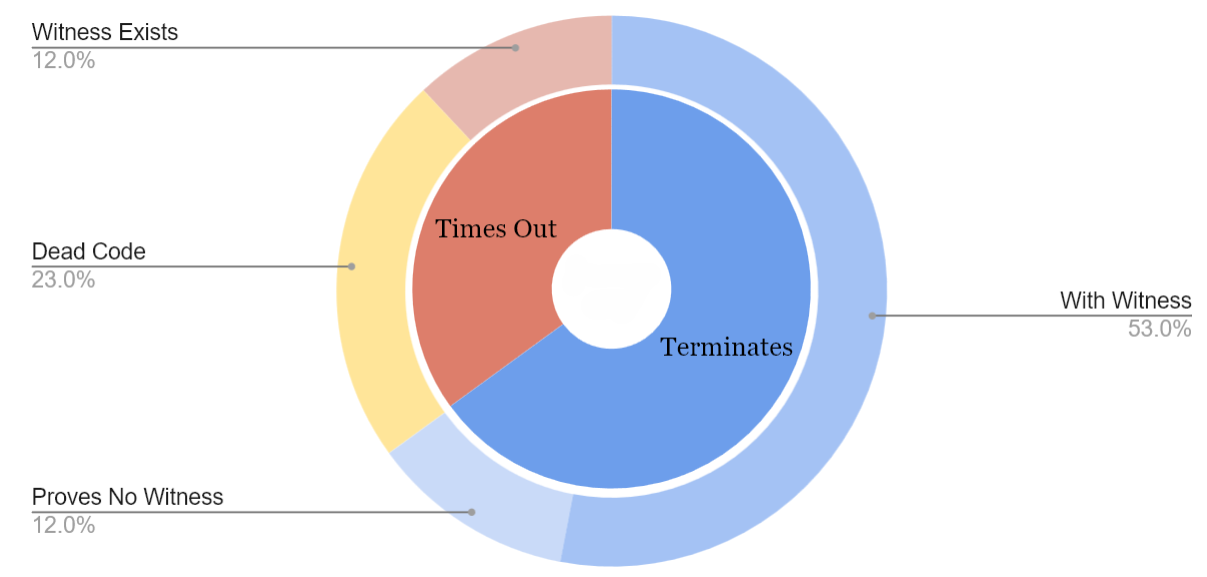
\includegraphics[width=1\textwidth]{Media/Figures/DFS_coverage}
\caption{DFS}
\end{subfigure}
%
\begin{subfigure}{0.45\textwidth}
\centering
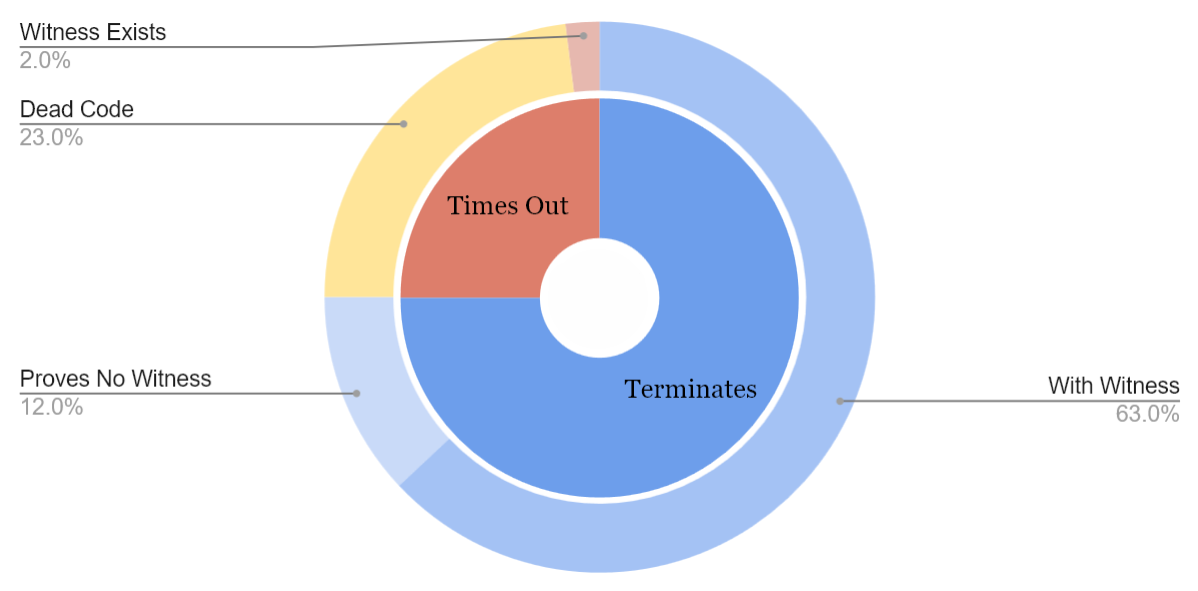
\includegraphics[width=1\textwidth]{Media/Figures/BDFS_coverage}
\caption{Bounded DFS}
\end{subfigure}

\vspace{1cm}

\begin{subfigure}{0.45\textwidth}
\centering

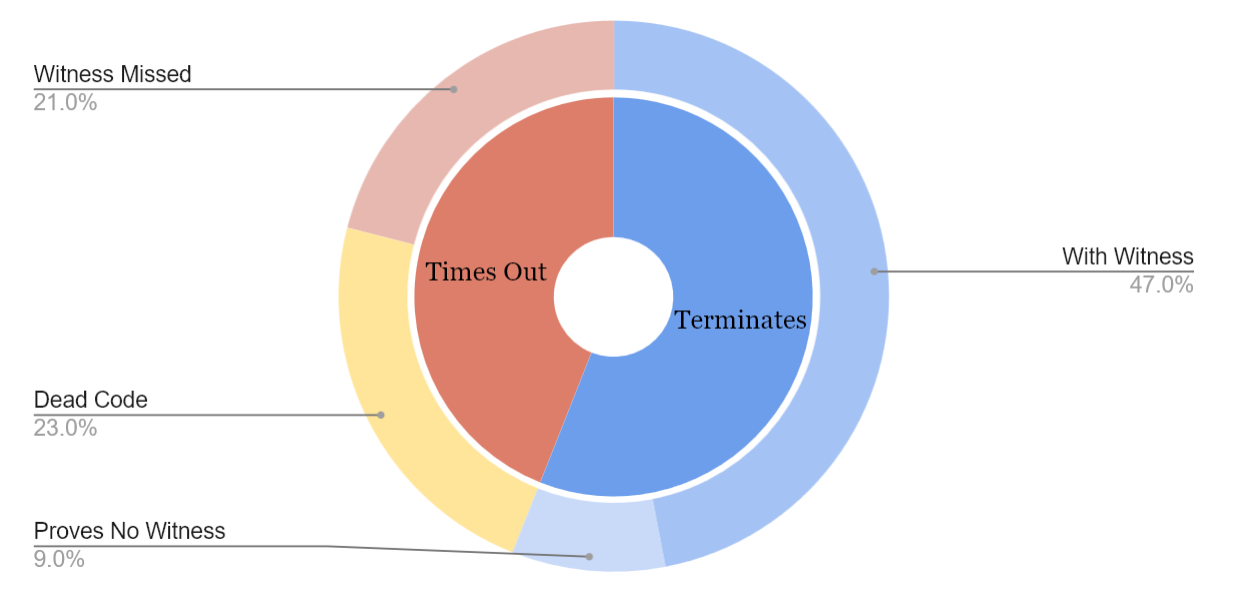
\includegraphics[width=1\textwidth]{Media/Figures/IDFS_coverage}
\caption{Interleaved DFS}
\end{subfigure}
%
\begin{subfigure}{0.45\textwidth}
\centering

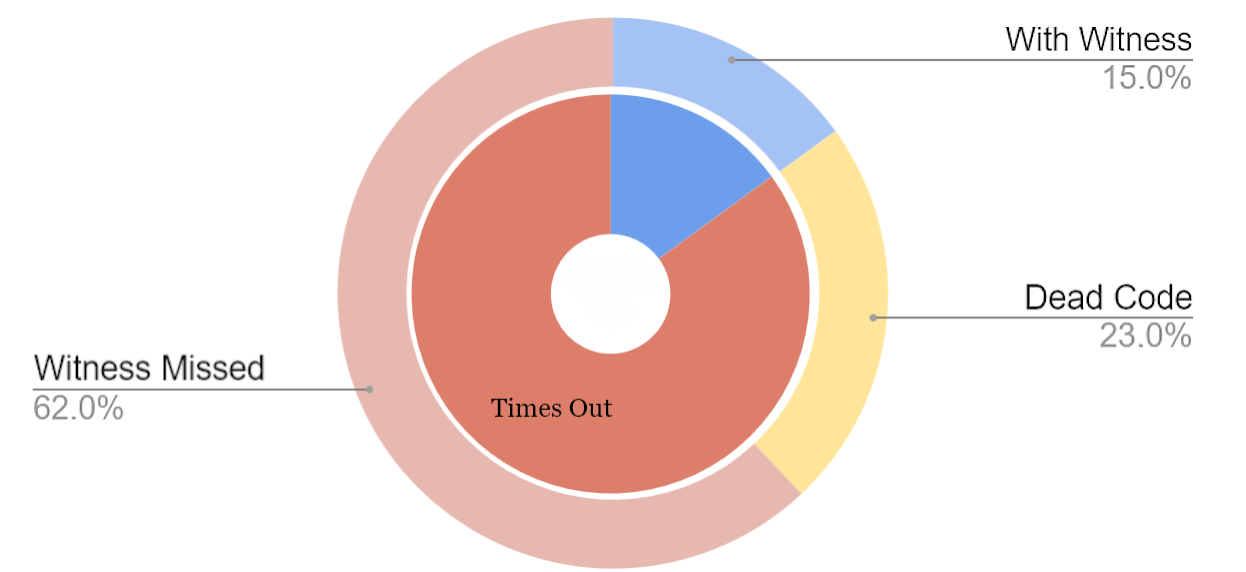
\includegraphics[width=\textwidth]{Media/Figures/BFS_coverage}
\caption{BFS}
\end{subfigure}

\caption{Search Procedure Coverage}
\label{fig:PieChart}
\end{figure}

The search procedure terminates either with a witness or proving no witness exists. A majority of programs terminated when using BDFS, DFS and IDFS, with BDFS meeting the 75\% target directly (\cref{fig:PieChart}). IDFS and BFS perform relatively poorly likely due to excessive memory usage (\cref{fig:SearchPerformance}). 

However, not all programs actually have an execution path leading to a dynamic type error. For example, errors within dead code cannot be found. I manually classified each failed program to check if a witness does exist, but was not found, or no witness exists. Of which, 89\% was found to be dead code and 5\% due to Hazel bugs\footnote{Being also present on the main branch, not just in my code.}, the bugs being excluded from the results. This gives only 2\% cases where BDFS failed to find an \textit{existing} witness; DFS and IDFS also meet the goal in failing in less than 25\% of cases.

\Cref{sec:SearchCategories} goes into further detail on categorising the programs which time out, and how this could be avoided.

\subsubsection{Witness \& Trace Size}
As predicted by the small-scope hypothesis, most programs admitted \textit{small} witnesses. And the depth first searches produce longer and more varied trace lengths, which allowed them, in combination with their lower memory overhead, to attain higher coverage (many witnesses were at a deeper depth than IDFS or BFS were able to reach).

However, there was no correlation (Pearson correlation \cite{PearsonCorrelation}) between witness sizes and trace sizes, even when normalised by the original deterministic evaluation trace lengths. This is likely because most errors are in the base cases, so few large witnesses are even found, with the noise from trace lengths to different programs' base cases dominating. 

\begin{figure}[h]\centering
\begin{tabular}{l|cccc}
& DFS & BDFS & BFS & IDFS\\
\hline
\textbf{Witness Size} Avg. & 1.1& 1.9&1.4&  2\\
Std. dev. & 1.2& 2.3&1.4&  2.3\\
\textbf{Trace size} Avg. & 33& 32& 11& 17\\
Std. dev. & 35& 33&2.4& 5
\end{tabular}
\caption{Witness \& Trace Sizes}
\label{fig:WitnessSize}
\end{figure}


\section{Critical Analysis}\label{sec:CriticalAnalysis}
This section discusses the implications of the previous results and delves deeper into the reasoning behind them. As a response to this analysis, many improvements have been devised, some of which have been implemented.
\subsection{Slicing}\label{sec:SlicingAnalysis}
\textit{Contribution slicing} produces large slices, highlight all branches, with much of the information is not particularly \textit{useful}, with much of it explaining why the use of \textit{subsumption} in subterms was valid, which is never directly related to type errors. As such,  I opted to use and evaluate synthesis and analysis slices for the task of explaining static errors more concisely. If a user were unsure as to why a sub-term is consistent with it's expected type, they can still select it to retrieve the slices.

The type slicing theory (\cref{sec:TypeSlicingTheory}) required that highlighted parts must form valid expressions or contexts.\footnote{Allows useful mathematical properties to be formalised.} But, some of the constructs highlighted are purely structural, not influencing the type, which could be omitted in practice. For example, bindings when the bound variable is dynamic or unused when typing the particular expression considered. This was a primary motivation in implementing slices via \textit{unstructured slices} (\cref{sec:UnstructuredCodeSlice}). I call these `ad-hoc' slices.

\Cref{fig:LetSliceOmitted} binds a integer \code{x}, but this variable is only used in one branch, where the type information for the \code{if} is already known from the other branch, so not included in the slice (highlighted in green). So, even though we selected\footnote{See the red cursor \& let expression filled in a darker colour.} the whole program, the let expression is omitted from the slice. Further, a contribution slice would be even more verbose here, highlighting \textit{everything}.\footnote{Both branches must be highlighted, and the conditional is only well-typed if \code{x} checks against an integer.}

\begin{figure}
\centering
\begin{subfigure}{0.45\textwidth}
\centering

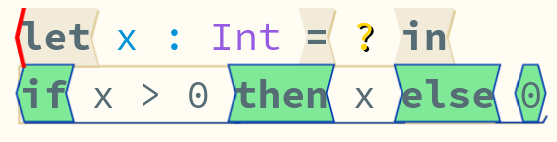
\includegraphics[width=1\textwidth]{Media/Figures/Unused_let}
\caption{Ad-hoc Slice: Let expression omitted}
\end{subfigure}$\qquad$
\begin{subfigure}{0.45\textwidth}
\centering

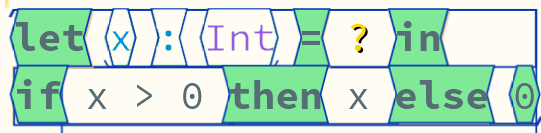
\includegraphics[width=1\textwidth]{Media/Figures/Unused_let_ordinary}
\caption{Ordinary Slice}
\end{subfigure}

\caption{An Ad-hoc Slice vs. Ordinary Slice}
\label{fig:LetSliceOmitted}
\end{figure}


\subsubsection{Error Slices}
When looking specifically at a \textit{type error}, there will be an inconsistency between the term's analysis and synthesis slices. Or, for synthesising branch statements, may also occur from multiple inconsistent branches (whom are \textit{all} synthesising). Meaning understanding the error requires looking at each of these.

However, some portions of the type may be consistent, not causing to the error. A form of type joining which extracts only the \textit{inconsistent parts} was therefore implemented. This became the default UI when clicking on a type error, see how branches synthesising or expecting inconsistent types \code{(Int, Int)} vs \code{(Int, String)} only highlights the right element in \cref{fig:ErrorSlice}.

\begin{figure}[h]
\begin{subfigure}{0.45\textwidth}
\centering

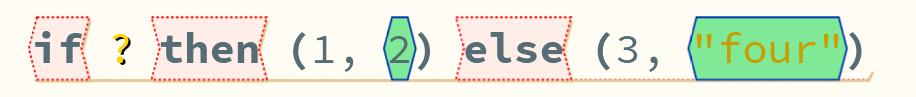
\includegraphics[width=1\textwidth]{Media/Figures/partially_inconsistent_branches}
\caption{Partially Inconsistent Branches}
\end{subfigure}$\qquad$
\begin{subfigure}{0.45\textwidth}
\centering

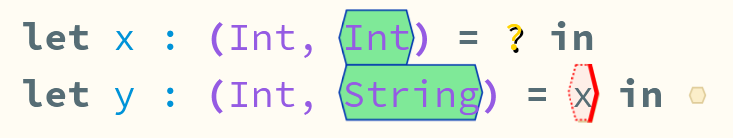
\includegraphics[width=1\textwidth]{Media/Figures/partially_inconsistent_expectations}
\caption{Partially Inconsistent Expectations}
\end{subfigure}

\caption{Error Slices}
\label{fig:ErrorSlice}
\end{figure}

Additionally, when the inconsistent parts are compound types, they must differ at their \textit{outermost} constructor (i.e. a \code{List} vs an \code{Int}). This can be considered the \textit{primary} cause of the error, inconsistencies deeper within the type were not the ones causing the error. These minimised slices (\cref{fig:MinimisedSlice}) were significantly smaller than naively combining the full slices (by 3x, see \fig{SlicingEffectiveness}); there would be an even larger ratio for more complex programs.\footnote{The corpus has few \textit{partially} inconsistent errors.}


\begin{figure}[h]
\begin{subfigure}{0.45\textwidth}
\centering

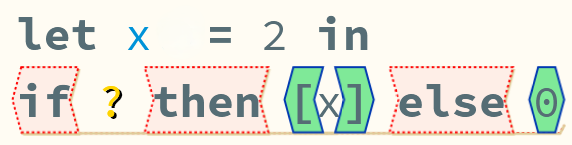
\includegraphics[width=1\textwidth]{Media/Figures/partially_inconsistent_compound}
\caption{Minimised Error Slice: Inner \code{Int} slice within list is omitted}
\end{subfigure}$\qquad$
\begin{subfigure}{0.45\textwidth}
\centering

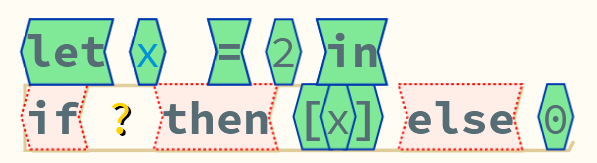
\includegraphics[width=1\textwidth]{Media/Figures/partially_inconsistent_compound_ordinary}
\caption{Ordinary Error Slice}
\end{subfigure}

\caption{Minimised Error Slices}
\label{fig:MinimisedSlice}
\end{figure}

\subsection{Structure Editing}\label{sec:StructureEditing}
Hazel uses a structure editor with an update calculus \cite{HazelStructureCalculus}. Statics are recalculated upon edits and even \textit{cursor movements}. \Cref{fig:SlicingPerformance}. While type checking with slices is still very fast, it is not so suitable for such a rapid use case.

Parsing and structural edit actions are made efficient\footnote{Constant time.} by use of a zipper data structure \cite{HuetZipper, OneHoleContext}. It might be possible to extend this zipper idea into the abstract syntax tree and it's statics (typing information), allowing local changes (and type changes) to propagate in the AST zipper. However, some local changes can propagate type changes \textit{non-locally} (e.g. inserting a new binding) which would require extensive recalculation of the typed AST. These non-local updates would be relatively rare. This is very complex and would require an entire rewrite of the Hazel statics, but would be beneficial for Hazel in general, not just type slicing.
  
\subsection{Static-Dynamic Error Correspondence}
\Cref{sec:StaticCastError} and \ref{sec:CastDependence} show how a static error that elaborates a cast failure, can be associated with a dynamic error whose cast error is dependent on this failed cast. This works well for most static type errors, which occur from inconsistent analysis and synthesis types.

However, static errors caused by synthesised branches being inconsistent, do not actually directly cause cast errors. Such errors will only be detected if both branches are used within a static context during the same evaluation path. The search procedure might find such cases if they exist, but cannot associate it back to the static error. Elaborating these terms does adds casts: on each branch to the dynamic type; these could be associated together with the error and tracked accordingly. 
  
\subsection{Categorising Programs Lacking Type Error Witnesses}
The 45 programs which timed out under the BDFS search procedure were manually inspected and classified as either:
\begin{itemize}
\item Witness Exists: BDFS failed to find an existing witness.
\item Dead Code: The error was in unreachable code by any type consistent instantiations. These then subclassified into:
\begin{itemize}
\item Pattern Cast Failure: An error was within a pattern matching branch, making the branch unreachable. These cast failures would be found by an extended pattern directed instantiation algorithm (\cref{sec:ExtendedPatternMatching}).\footnote{Where inconsistent patterns would be attempted, and subsequently reduced to concrete cast failures in expressions.}
\item Wildcards: Trivially dead code bound to no variable, i.e. a 
\item Non-Trivial: Dead code which is less easily detectable. There was only one example which was due to infinite recursion for all inputs.
\end{itemize}
\item Hazel Bugs: Evaluation errors encountered stemming from \textit{unboxing bugs} in the main branch of Hazel. These were excluded from the statistics.
\end{itemize}
Three (paraphrased) examples given in \cref{fig:FailureExamples}, with the full classification in \texttt{failure-classification.txt}. 

\begin{figure}[h]
\centering
\begin{subfigure}{1\textwidth}
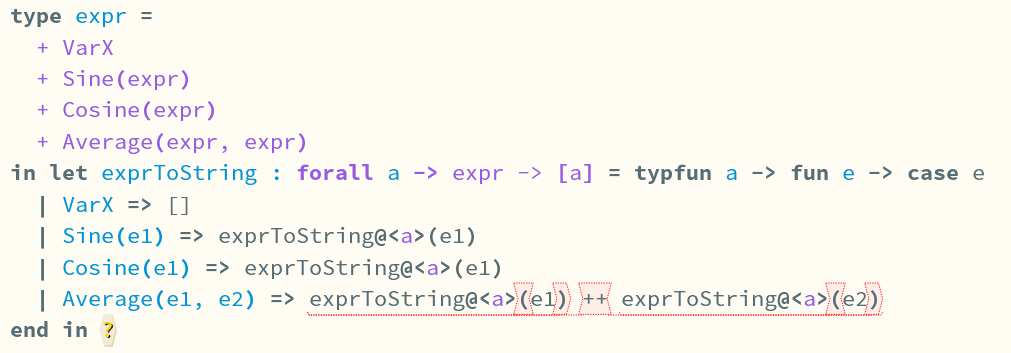
\includegraphics[width=1\textwidth]{Media/Figures/witness_exists}

Depth-first bias caused the procedure to try mostly permutations of \code{Sine(...)} and \code{Cosine(...)}. The error was on the \code{Average(...)} branch, not found within the time limit.
\caption{Witness Exists: prog2270.typed.hazel}
\end{subfigure}

\begin{subfigure}{1\textwidth}
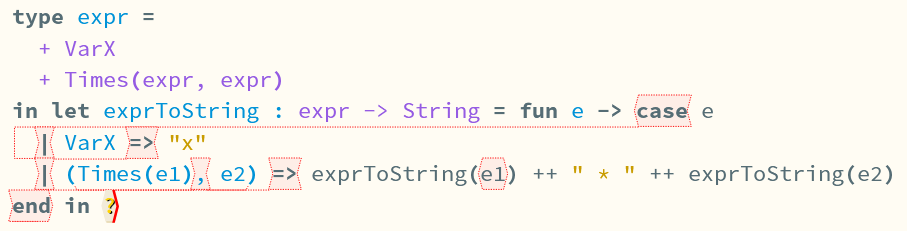
\includegraphics[width=0.8\textwidth]{Media/Figures/dead_code_pattern_instantiation}
A tuple pattern is used when an \code{expr} is expected. Instantiation only tries value of type \code{expr}. Further, another error exists inside this inaccessible branch.
\caption{Dead Code -- Wildcard: prog0080.typed.hazel}
\end{subfigure}

\begin{subfigure}{0.7\textwidth}
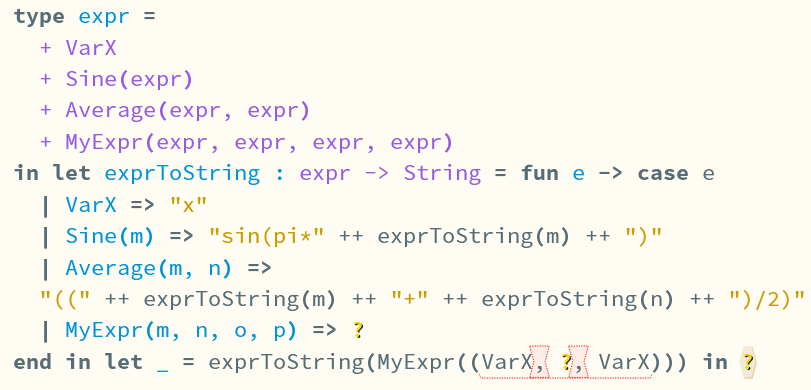
\includegraphics[width=1\textwidth]{Media/Figures/dead_code_wildcard}
Product arity inconsistency is present in inaccessible code bound to the wildcard pattern.
\caption{Dead Code -- Pattern Cast Failure: prog0339.typed.hazel}
\end{subfigure}
\caption{(Paraphrased) Failure Examples}
\label{fig:FailureExamples}
\end{figure}

\label{sec:SearchCategories}
\subsubsection{Non-Termination, Unfairness, and Search Order}
DFS is fast, but has significant insurmountable issues with non-termination, resulting in it having worse coverage than BDFS (\cref{fig:PieChart}). Any time evaluation goes into an infinite loop, no more instantiations can be explored. Bounded DFS, BFS, and interleaved DFS, were implemented in response to this. With BDFS performing best due to preference of evaluation over instantiation (and it's lesser memory footprint \cref{fig:SearchPerformance}).

BFS and IDFS would do significantly better if the search algorithm was tweaked to less frequently wrap deeper in the search tree, effectively reducing the \textit{cost} of evaluation. For example, it could wrap evaluation in one extra search depth only once every 10 steps, allowing 10 steps of evaluation to be explored for every instantiation. This is a delicate balancing act.
\subsubsection{Repeated Instantiations}
Sometimes, a hole can get repeatedly refined to increasingly specific types without ever actually causing a cast error, see \cref{fig:InfiniteInstantiations}. This situation would be caught statically, but cannot actually directly lead to a cast error.\footnote{So is not classified as having a witness under these semantics.} 

\begin{figure}[h]
\centering
See the `safe' list example from Seidel.
\caption{Instantiations of Increasingly Specific Types Loop}
\label{fig:InfiniteInstantiations}
\end{figure}

\subsubsection{Dead Code}
Dead code may contain or be involved in static type errors, but is unreachable dynamically, such static errors have no dynamic witness. Dead code detection \cite{DeadCodeDetection} could alert the user of this.

Pattern matching instantiation helps

\subsubsection{Dynamic Match Statements}
Current instantiation removes failed casts found here...

\subsubsection{Dynamically Safe Code}
Some code with static errors is inherently dynamically safe, the typical example being \code{if true then 0 else "str"}. These should have \textit{no} dynamic witness. 

Early versions of the search procedure would incorrectly detect cast failures that were inserted statically during elaboration, but weren't actually causing dynamic, leading to dynamically safe code being incorrectly asserted as an error. \Cref{sec:CastFailureDetection} detailed how cast errors were detected \textit{correctly}.

\subsubsection{Cast Laziness}
Currently only allow ground type inconsistency. Not a single example in the codebase had non-ground inconsistency!

\subsubsection{Combinatorial Explosion}
Some programs have cast errors that are intricately dependent on specific instantiations. These casts only manifest within a branch which requires very specific inputs. When multiple holes are involved, this is an even bigger issue, as the search space increases exponentially in the number of holes.

The fact the a large proportion of programs which failed due to insufficient time or space had lower code coverage (\cref{fig:CodeCoverage}), suggests that this might be the reason behind a large proportion of the failures.

\begin{figure}\centering
Pair of single inputs leading to cast error
\caption{Branch Requiring Specific Instantiations}
\label{fig:SpecificInstantiations}
\end{figure}

Combinatorial explosion clearly has a particularly big affect on IDFS and BFS, who prioritise trying different instantiations over evaluating. The space usage then becomes a big bottleneck on speed, causing the witnesses (which have been instantiated by now) to not actually evaluate far enough to detect the error. The balance between instantiating vs evaluation could be tweaked to improve the two.

\subsection{Improving Code Coverage}
\label{sec:EvalHoleInstantiation}
Of the discussed classes of programs lacking a type error witness (\cref{sec:SearchCategories}), only one actually had concrete witnesses that were not found within the time limit. This was due to the solution being a small number of possible instantiations within a large search space. I pointed out that that the search procedure had lower code coverage in these situations, and the possible cast error is likely to be in portions of the code that were \textit{missed}.

These errors require rather specific, often interdependent, inputs to be missed by the current search procedure. Therefore, it is likely that programmers are \textit{also} more likely to not notice errors (in dynamic code), or not understand the errors (in static code).\footnote{After all, spotting the error might require understanding interdependent inputs.}

Intelligently directing hole instantiations to better explore the code would help. Purely structural pattern-directed instantiation was discussed in \cref{sec:ExtendedPatternMatching}, but was not found to significantly increase code coverage nor reduce failed searches. This might be because the examples involving very specific inputs in the corpus happen to be mostly to do with \textit{if} statements, rather than \textit{match} statements.

In order to extend this structural pattern-directed instantiation to worth also with base types (integers), requires more efficient ways to representing constraints. To extend this to include floats, inequalities, list lengths, etc. requires full-blown symbolic execution \cite{SymbolicExecutionSurvey}. 

Symbolic execution and program test generation is a well-researched area with numerous dedicated constraint solvers \cite{CITE MANY HERE} and translations to theories for SMT solvers \cite{CITE}. However, even without this, the search procedure still retains a high coverage, finding most errors.

\begin{figure}\centering
Proportions found using iterative deepening under the time limit. Also, code coverage comparison.
\caption{Pattern-directed Hole Instantiation Using Iterative Deepening}
\end{figure}

\section{Holistic Evaluation}
\label{sec:HolisticEvaluation}

This section considers a number of examples of ill-typed Hazel programs, \textit{holistically} and \textit{qualitatively} evaluating how a user might use the three features and the existing bidirectional type error error localisation \cite{HazelErrors} to debug the errors. 


\subsection{Type Error Localisation in Hazel}
\textbf{Ref to each example here...}

Hazel has three types of errors which can be addressed by this project:\footnote{Others being syntax errors, unbound names, duplicate labels, deferrals, or redundant pattern matches.} \textit{inconsistent expectations} (where a term's analytic and synthetic types are inconsistent), \textit{inconsistent branches }(where branches are synthetic and inconsistent, this also applies to values in a list literal), and \textit{inexhaustive match} warnings. 

The witness search procedure can easily associate \textit{inconsistent expectation} errors with a witness: a dynamic cast error and trace. Inconsistent branches will be detected by the procedure, but are not automatically associated to the static error. Explaining inexhaustive match statements was not a core aim of this project, but the indeterminate evaluation can be adapted for this anyway (see the \texttt{inexhaustive-matches} branch \textbf{TODO}). Static generation of counter-examples to match statement exhaustivity is already a solved problem \textbf{(CITE)}, and is under development for Hazel.\footnote{Indeterminate evaluation is very inefficient in comparison. This counter-examples logic is useful for directing hole instantiation (\cref{sec:EvalHoleInstantiation}).}

Bidirectional type error localisation is generally very good \cite{BidirectionalTyping}. Type slicing can provide an explanation of where type expectations in the error were sourced. However, there are still cases where the error highlighted is not the actual location of the error.\footnote{Also, Hazel has plans to introduce global inference in the future, where correct localisation becomes even more difficult.} These often arise due to \textit{misunderstanding} of the programmer about the actual types of the code. Fundamentally, there is \textit{no} way for a type system to always correctly localise such errors. Use of the Hazel context inspector and type slices can help clear these misunderstandings.

Additionally, some errors might require changes to \textit{multiple} parts of the code \cite{StudentTypeErrorFixes}. Unlike most languages, Hazel \textit{does} allow \textit{multiple} errors to be detected \textit{completely} \cite{HazelErrors}. However, these errors are typically \textit{not associated} together.\footnote{Except for \textit{inconsistent branches} errors.} Type slicing can give a more complete view of regions that might contain the multiple parts pertaining to the \textit{actual} error.

Finally, there may be errors in \textit{dynamic regions} of the code. These are not found statically. The search procedure tests dynamic code for such type errors automatically. Indeterminate evaluation could also, in future, be used to perform property testing of code, in the sense of SmallCheck \cite{SmallCheck}. Adding annotations to find type errors is time-consuming, often a large number of, concrete, annotations are required to make the code static enough to detect errors. For example, \cref{fig:HalfAnnotated} shows a partially annotated program, which \textit{still} doesn't provide enough type information to detect the error statically.

\subsection{Examples}
Merge these examples into the paragraphs above?? Want an example for each. All the examples can apply to dynamic errors.

\begin{figure}[h]
Error in the @ operator. Due to annotation, search procedure can help give reasoning.
\begin{lstlisting}
let map : (Int -> Int) -> [Int] -> [Int] = fun f -> fun l -> case l 
  | [] => []
  | x::xs => f(x) @ map(f)(xs)
end in  
\end{lstlisting}
\caption{Inconsistent Expectations Example}
\end{figure}

\begin{figure}[h]
Error in the @ operator. But arises as inconsistent branches. Use type slicing to work out types of branches. \textbf{use search procedure to find location of the actual error! via a cast slice!}
\begin{lstlisting}
let map = fun f -> fun l -> case l 
  | [] => []
  | x::xs => f(x) @ map(f)(xs)
end in  
\end{lstlisting}
\caption{Inconsistent Branches Example}
\end{figure}

\begin{figure}
More difficult, non-local example where it's harder to work out the types of the branches immediately:
\begin{lstlisting}
let f = fun x -> x + 1 in
let g = fun x -> x ++ "a" in 
let broken = fun x -> if x then f(x) else g(x)
\end{lstlisting}
\caption{Inconsistent Branches Example 2}
\end{figure}

\begin{figure}
\textbf{COMPLEX ERROR}
Trying to use the curried fold function with uncurried add function.
\begin{lstlisting}
let fold : ((Int, Int) -> Int) -> Int -> [  ] -> Int = fun f -> fun init -> fun l -> 
  case l 
    | [] => init 
	| x::xs => f(x, fold(f)(init)(xs)) 
  end 
in
let add = fun x -> fun y -> x + y in
let sum = fold(add)(0) in
sum([1,2,3])
\end{lstlisting}
\caption{Confused Currying Example}
\label{fig:TastyCurry}
\end{figure}


\begin{figure}
\begin{subfigure}{.5\textwidth}
\centering
Type error is NOT spotted
\begin{lstlisting}
let map : (? -> ?) -> [?] -> [?] = fun f -> fun l -> case l 
  | [] => []
  | x::xs => f(x) @ map(f)(xs) 
end in   
\end{lstlisting}
\caption{Program}
\end{subfigure}

\begin{subfigure}{.5\textwidth}\centering
\begin{lstlisting}
let map : (? -> ?) -> [?] -> [?] = fun f -> fun l -> case l 
  | [] => []
  | x::xs => f(x) @ map(f)(xs) 
end in   
\end{lstlisting}
\caption{Static Regions (Contibution Slice)}
\end{subfigure}
\caption{Partially Annotated Program}
\label{fig:HalfAnnotated}
\end{figure}

\subsection{Usability Improvements}\label{sec:UIImprovements}
As designing an intuitive user interface was not a core goal, the actual use of the features can be quite awkward or unintuitive. Below, I propose various improvements, for which the architecture, of both Hazel and the newly implemented features, is sufficiently abstract and flexible to easily support:\footnote{Some of which were detailed in the Implementation chapter.}

\begin{figure}\centering
Screenshot the Hazel context inspector, including a case with an error, and with analysing and synthesising types.
\caption{The Hazel Context Inspector}
\label{fig:ContextInspector}
\end{figure}

\begin{itemize}
\item Displaying type slices only \textit{upon request} using the Hazel \textit{context inspector}, which displays the \textit{analysing} and \textit{synthesising} types of the selected expression, see \cref{fig:ContextInspector}. This can also improve live-editing performance (see \cref{sec:StructureEditing}).
\item A UI allowing the user to deconstruct type slices to query, for example: if a term has a function type, they could select the \textit{return type} and get only the part of the slice relevant to that.
\item Graphs visualising cast dependence (\cref{sec:CastDependence}). Showing the \textit{execution} context that leads to a cast error; these would be more concise summaries than full evaluation traces.
\item Graphs visualising the search procedure's execution traces and instantiations.
\item Key bindings to more quickly cycle through indeterminate evaluation instantiation paths.
\item Integration with the Hazel stepper,\footnote{The inbuilt trace visualiser, which also allows arbitrary evaluation order.} which could also allow (optionally) user-directed hole instantiations. The Hazel stepper could also be improved to allow other standard techniques like stepping over functions calls.
\end{itemize}